%XeLaTeX
\documentclass[aspectratio=169,10pt,xcolor=table]{beamer}
\usetheme[progressbar=frametitle, sectionpage=none, numbering=fraction, block=fill]{metropolis}

\usepackage{fontspec}
\usepackage{polyglossia}
\setmainlanguage{greek}
\setotherlanguage{english}
\setmainfont{Arial}
\setsansfont{Arial}
\setmonofont{Consolas}[Scale=MatchLowercase]

\usepackage{graphicx}
\graphicspath{{figures/}{../Report/figures/}}
\usepackage{amsmath}
\usepackage{amssymb}
\usepackage{booktabs}
\usepackage{tikz}
\usetikzlibrary{positioning, arrows.meta, fit, calc}
\usepackage{pgfplots}
\pgfplotsset{compat=1.18}

% Colours (diagram fills follow the report's TikZ figures)
\definecolor{navy}{HTML}{1F3A5F}
\definecolor{accent}{HTML}{B03A2E}
\setbeamercolor{palette primary}{bg=navy, fg=white}
\setbeamercolor{frametitle}{bg=navy, fg=white}
\setbeamercolor{progress bar}{fg=accent, bg=accent!20}
\setbeamercolor{alerted text}{fg=accent}
\setbeamercolor{background canvas}{bg=white}
\setbeamercolor{normal text}{fg=black!85}
\setbeamercolor{block title}{bg=navy!12, fg=navy}
\setbeamercolor{block body}{bg=navy!4}
\setbeamertemplate{section in toc}{\leavevmode{\usebeamercolor[fg]{itemize item}\usebeamertemplate{itemize item}}\hspace{0.6em}\inserttocsection\par}

\title{``Talking Heads'': Πρόβλεψη Φωνημάτων από Βίντεο}
\author{Βαπόρης Δημήτριος}
\hypersetup{pdftitle={Talking Heads: Πρόβλεψη Φωνημάτων από Βίντεο}, pdfauthor={Βαπόρης Δημήτριος}}

\newcommand{\ph}[1]{/#1/}

\tikzset{
  blk/.style={draw=black!60, thick, rounded corners=2pt, align=center, inner sep=2pt},
  arr/.style={-{Latex[length=1.8mm]}, thick},
  dimlbl/.style={font=\tiny, text=black!60},
  note/.style={font=\scriptsize, text=black!65},
  framestack/.style={inner sep=0pt, draw=white, line width=0.8pt},
  word/.style={draw=black!50, rounded corners=2pt, fill=#1, minimum width=17mm,
               minimum height=8mm, font=\normalsize\bfseries},
}

\begin{document}

% =====================================================================
% Title page (layout follows the report's cover page)
% =====================================================================
\begin{frame}[plain]
  \centering
  \setlength{\parskip}{0pt}
  \includegraphics[height=12mm]{banner-horizontal-black300ppi.png}\par
  \vspace{8pt}
  {\small\bfseries Τμήμα Ηλεκτρολόγων Μηχανικών και Μηχανικών Υπολογιστών}\par
  \vspace{4pt}
  {\footnotesize\bfseries Τομέας Ηλεκτρονικής και Υπολογιστών}\par
  \vspace{3pt}
  {\footnotesize\bfseries Εργαστήριο Επεξεργασίας Πληροφοριών και Υπολογισμών}\par
  \vspace{14pt}
  {\normalsize\bfseries Διπλωματική Εργασία}\par
  \vspace{6pt}
  {\Large\bfseries\color{navy} ``Talking Heads'': Πρόβλεψη Φωνημάτων από Βίντεο}\par
  \vspace{14pt}
  {\footnotesize
  \renewcommand{\arraystretch}{1.25}
  \begin{tabular}{r|l}
    \textbf{Όνομα} & Βαπόρης Δημήτριος \\
    \textbf{Α.Ε.Μ.} & 10625 \\
    \textbf{Email} & dvaporis@ece.auth.gr \\
    \textbf{Επιβλέπων Καθηγητής} & Ντελόπουλος Αναστάσιος \\
  \end{tabular}}\par
  \vspace{12pt}
  {\small\bfseries Εαρινό Εξάμηνο 2026}\par
\end{frame}

\begin{frame}{Περιεχόμενα}
  \tableofcontents
\end{frame}

% =====================================================================
\section{Εισαγωγή}
% =====================================================================

\begin{frame}{Ορισμός του Προβλήματος}
  \begin{columns}[c]
    \begin{column}{0.56\textwidth}
      \begin{itemize}
        \item Lip reading: αναγνώριση ομιλίας από βίντεο
        \item \alert{VSR}: αποκλειστικά οπτικά στοιχεία
        \item \alert{AVSR}: οπτικά και ακουστικά στοιχεία
        \item Δυσκολία: «bin» και «pin» φαίνονται ίδια
        \item Με θόρυβο: κρίση αξιοπιστίας κάθε τροπικότητας
        \item Εφαρμογές: βαρήκοοι, Augmented Reality, θορυβώδεις χώροι
      \end{itemize}
    \end{column}
    \begin{column}{0.42\textwidth}
      \centering
      \begin{tikzpicture}[font=\scriptsize]
        \node[inner sep=0pt] (frame) at (0,0) {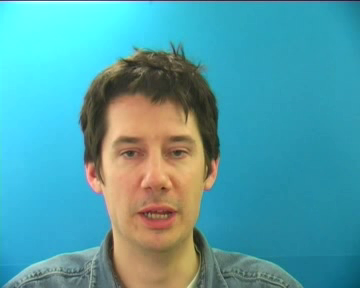
\includegraphics[width=26mm]{grid_bbaf2n_f49.png}};
        \node[note, below=1mm of frame] (flbl) {βίντεο};
        \draw[thick, purple!70!black, domain=0:2.4, samples=150, smooth]
          plot ({2.45+\x*0.75}, {0.45*sin(14*\x r)*exp(-0.8*(\x-1.2)^2)});
        \node[note, anchor=north, align=center] (albl) at (flbl.north -| 3.35,0) {ηχητικό σήμα\\(θορυβώδες ή απόν)};
        \node[blk, fill=teal!12, minimum width=50mm, minimum height=8mm] (model) at (1.7,-2.75)
          {\textbf{Μοντέλο VSR / AVSR}};
        \node[font=\small\itshape, text=navy] (txt) at (1.7,-3.75) {``bin blue at f two now''};
        \draw[arr] (flbl.south) -- (model.north -| flbl.south);
        \draw[arr] (albl.south) -- (model.north -| albl.south);
        \draw[arr] (model) -- (txt);
      \end{tikzpicture}
    \end{column}
  \end{columns}
\end{frame}

\begin{frame}{Διαθέσιμες Μέθοδοι \& Η Συγκεκριμένη Εργασία}
  \small
  \begin{columns}[T]
    \begin{column}{0.47\textwidth}
      \begin{block}{Διαθέσιμες Μέθοδοι}
        \begin{itemize}
          \item LipNet, WLAS: 3D CNN + RNN/attention
          \item AV-HuBERT, Auto-AVSR: προεκπαίδευση μεγάλης κλίμακας
          \item VALLR: φωνήματα, έπειτα λέξεις μέσω κατάλληλα fine-tuned LLM
        \end{itemize}
      \end{block}
    \end{column}
    \begin{column}{0.47\textwidth}
      \begin{block}{Η Συγκεκριμένη Εργασία}
        \begin{itemize}
          \item Εστίαση: πρόβλεψη φωνημάτων ανά frame
          \item Visual μοντέλο: βουβό βίντεο χειλιών
          \item Audiovisual μοντέλο: παραμορφωμένο βίντεο και θορυβώδης ήχος
          \item 3 πειράματα στο GRID dataset
        \end{itemize}
      \end{block}
    \end{column}
  \end{columns}
  \vfill
  \centering
  \begin{tikzpicture}[font=\small, node distance=12mm]
    \node[blk, fill=blue!8, minimum width=30mm, minimum height=9mm] (in) {Βίντεο (+ ήχος)};
    \node[blk, fill=accent!15, draw=accent, minimum width=30mm, minimum height=9mm, right=of in] (ph) {\textbf{Φωνήματα}};
    \node[blk, dashed, fill=black!3, minimum width=30mm, minimum height=9mm, right=of ph] (w) {Λέξεις / φράσεις};
    \draw[arr] (in) -- (ph);
    \draw[arr] (ph) -- (w);
    \node[below=1mm of w, note] {αλγοριθμικά (GRID) / LLM};
  \end{tikzpicture}
\end{frame}

% =====================================================================
\section{Τεχνικό Υπόβαθρο}
% =====================================================================

\begin{frame}{Φωνήματα και Visemes}
  \begin{columns}[c]
    \begin{column}{0.56\textwidth}
      \begin{itemize}
        \item \alert{Φώνημα}: η ελάχιστη μονάδα φωνής
        \item Π.χ. \ph{b} στην αρχή της λέξης «bat»
        \item \alert{Viseme}: φωνήματα με ίδια όψη χειλιών
        \item Visemes: πληροφορία τόπου, όχι τρόπου εκφοράς
        \item Ο ήχος διαχωρίζει φωνήματα ίδιου viseme
        \item Ομαδοποίηση: τόπος και τρόπος εκφοράς, έμφωνο/άφωνο
      \end{itemize}
    \end{column}
    \begin{column}{0.42\textwidth}
      \centering
      \begin{tikzpicture}[font=\small]
        \node[blk, fill=purple!8, minimum width=11mm, minimum height=7mm] (p) at (0, 1.3) {\ph{p}};
        \node[blk, fill=purple!8, minimum width=11mm, minimum height=7mm] (b) at (0, 0)   {\ph{b}};
        \node[blk, fill=purple!8, minimum width=11mm, minimum height=7mm] (m) at (0,-1.3) {\ph{m}};
        \node[inner sep=0pt] (lips) at (2.8,0) {
\includegraphics[width=19mm]{lips_bbaf2n_f24.png}};
        \draw[arr] (p.east) -- ($(lips.west)+(0,0.5)$);
        \draw[arr] (b.east) -- (lips.west);
        \draw[arr] (m.east) -- ($(lips.west)+(0,-0.5)$);
        \node[below=1mm of lips, note, align=center] {ίδια όψη χειλιών (διχειλικά)\\[1pt] {\tiny\ph{b} του «bin», bbaf2n frame 24}};
        \node[left=1mm of p, note] {«pat»};
        \node[left=1mm of b, note] {«bat»};
        \node[left=1mm of m, note] {«mat»};
      \end{tikzpicture}
    \end{column}
  \end{columns}
\end{frame}

% =====================================================================
\section{Μεθοδολογία}
% =====================================================================

\begin{frame}{Προεπεξεργασία Δεδομένων}
  \begin{columns}[c]
    \begin{column}{0.52\textwidth}
      \centering
      \includegraphics[width=\linewidth]{bbaf2n_frame0049_comparison.jpg}\\[1mm]
      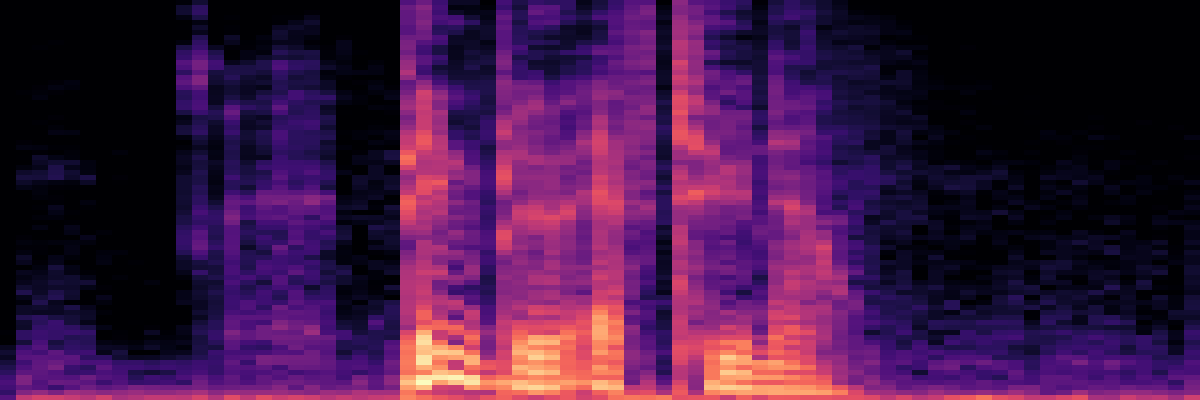
\includegraphics[width=\linewidth, height=13mm]{mel_bbaf2n.png}\\[0.5mm]
      {\tiny\color{black!60} bbaf2n.mpg: εξαγωγή χειλιών (frame 49) και log Mel-Spectrogram}
    \end{column}
    \begin{column}{0.46\textwidth}
      \textbf{Βίντεο}
      \begin{itemize}
        \item MediaPipe Face Landmarker: τοπόσημα χειλιών
        \item Bounding box με padding 30\%
        \item Resize σε $224\times224$, τελικά $96\times96$
        \item Περιοχή περίπου 1.6\% του αρχικού frame
      \end{itemize}
      \textbf{Ήχος}
      \begin{itemize}
        \item Log Mel-Spectrogram, 80 φίλτρα mel
        \item Βήμα $N_h = f_s/f_v$: ευθυγράμμιση με frames του βίντεο
      \end{itemize}
    \end{column}
  \end{columns}
\end{frame}

\begin{frame}{Visual Μοντέλο}
  \centering
  \begin{tikzpicture}[font=\scriptsize, node distance=7mm]
    \node[framestack] (i3) at (0.36,0.36) {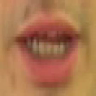
\includegraphics[width=11mm]{lips_bbaf2n_f49.png}};
    \node[framestack] (i2) at (0.18,0.18) {
\includegraphics[width=11mm]{lips_bbaf2n_f24.png}};
    \node[framestack] (i1) at (0,0)       {
\includegraphics[width=11mm]{lips_bbaf2n_f00.png}};
    \node[below=1mm of i1, note, align=center] {βίντεο χειλιών\\$T\times3\times96\times96$};

    \node[blk, fill=blue!8, minimum width=27mm, minimum height=17mm, anchor=west] (fe) at (1.6,0.18)
      {\textbf{Conv3D Frontend}\\[1pt] 3 depthwise separable\\ 3D blocks\\ $3{\to}32{\to}64{\to}128$\\ pool $3{\times}3$ + Linear};
    \node[blk, fill=blue!8, minimum width=15mm, minimum height=17mm, right=of fe] (pe)
      {Positional\\Encoding};
    \node[blk, fill=green!10, minimum width=17mm, minimum height=17mm, right=of pe] (enc)
      {\textbf{BiLSTM}\\ 2 στρώσεις\\[1pt] \tiny(Sequence\\ \tiny Encoder)};
    \node[blk, fill=orange!12, minimum width=20mm, minimum height=17mm, right=of enc] (head)
      {\textbf{Classification}\\ \textbf{Head}\\[1pt] Linear $\to N_p{+}1$};

    \draw[arr] (i2.east -| i3.east) ++(0.05,0) -- (fe.west);
    \draw[arr] (fe) -- node[above, dimlbl] {$T{\times}h$} (pe);
    \draw[arr] (pe) -- node[above, dimlbl] {$T{\times}h$} (enc);
    \draw[arr] (enc) -- node[above, dimlbl] {$T{\times}2h$} (head);

    % per-frame output
    \foreach \t [count=\k] in {$\varnothing$, b, ɪ, ɪ, $\varnothing$, n} {
      \node[draw=black!40, fill=white, minimum size=4.5mm, inner sep=0pt, font=\scriptsize]
        (o\k) at ($(head.south) + (-1.375 + 0.55*\k, -1.05)$) {\t};
    }
    \draw[arr] (head.south) -- (head.south |- o1.north);
    \node[below=0.5mm of o3.south east, note] {έξοδος: ένα φώνημα ανά frame};
  \end{tikzpicture}

  \small
  \begin{columns}[T]
    \begin{column}{0.48\textwidth}
      \begin{itemize}
        \item 3D συνέλιξη: εμφάνιση και κίνηση χειλιών
        \item Depthwise separable: έως $22\times$ λιγότερες παράμετροι
        \item Χρονικό stride 1: διατήρηση όλων των frames
      \end{itemize}
    \end{column}
    \begin{column}{0.48\textwidth}
      \begin{itemize}
        \item Frontend: receptive field 7 frames
        \item BiLSTM: παρακείμενο (context) παρελθόντος και μέλλοντος
        \item Έξοδος: φωνήματα + blank ανά frame
      \end{itemize}
    \end{column}
  \end{columns}
\end{frame}

\begin{frame}{Audiovisual Μοντέλο}
  \centering
  \begin{tikzpicture}[font=\scriptsize]
    % inputs
    \node[framestack] (v3) at (0.86,1.16) {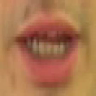
\includegraphics[width=10mm]{lips_bbaf2n_f49.png}};
    \node[framestack] (v2) at (0.68,0.98) {
\includegraphics[width=10mm]{lips_bbaf2n_f24.png}};
    \node[framestack] (v1) at (0.5,0.8)   {
\includegraphics[width=10mm]{lips_bbaf2n_f00.png}};
    \node[inner sep=0pt] (mel) at (0.85,-0.8) {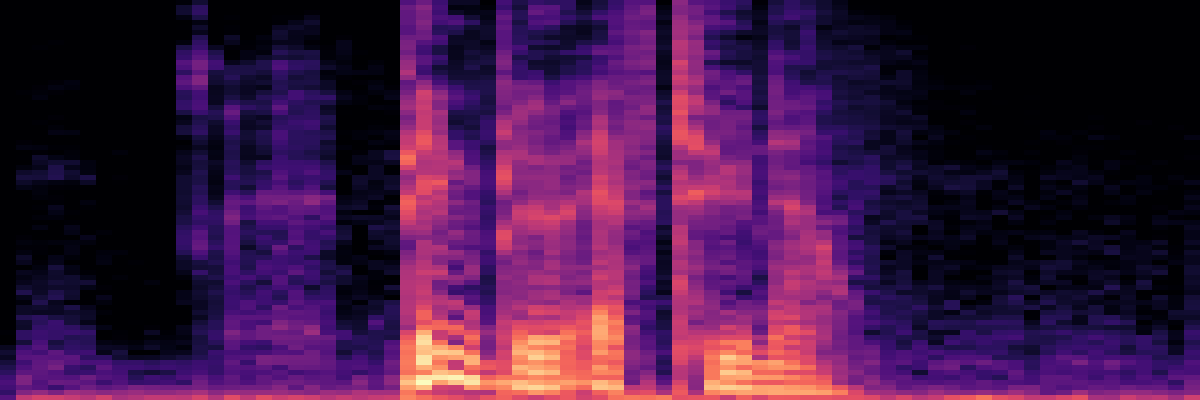
\includegraphics[width=17mm, height=10mm]{mel_bbaf2n.png}};
    \node[below=0.5mm of mel, dimlbl] {log Mel-Spectrogram};

    % frontends
    \node[blk, fill=blue!8, minimum width=21mm, minimum height=12mm] (vfe) at (3.2,0.8)
      {\textbf{Conv3D}\\ \textbf{Frontend}\\ + Pos. Enc.};
    \node[blk, fill=purple!8, minimum width=21mm, minimum height=12mm] (afe) at (3.2,-0.8)
      {\textbf{AudioMel}\\ \textbf{Frontend (2D)}\\ + Pos. Enc.};

    % cross-modal attention
    \node[blk, fill=teal!10, minimum width=21mm, minimum height=31mm] (xatt) at (5.95,0) {};
    \node[font=\scriptsize\bfseries, align=center] at (5.95,0) {Cross-modal\\Attention};
    \node[blk, thin, fill=white, minimum width=17mm, minimum height=6.5mm] (va) at (5.95,0.95) {$F_v \leftarrow F_a$};
    \node[blk, thin, fill=white, minimum width=17mm, minimum height=6.5mm] (av) at (5.95,-0.95) {$F_a \leftarrow F_v'$};

    % fusion
    \node[blk, fill=teal!22, minimum width=22mm, minimum height=31mm, align=center] (fus) at (8.75,0)
      {\textbf{Reliability-}\\ \textbf{gated Fusion}\\[4pt] $g_v F_v' + g_a F_a'$};
    \node[blk, fill=yellow!15, draw=black!40, thin] (rel) at (8.75,2.3) {σήματα αξιοπιστίας $r_v(t),\ r_a(t)$};

    % encoder and head
    \node[blk, fill=green!10, minimum width=15mm, minimum height=13mm] (enc) at (11.1,0)
      {\textbf{BiLSTM}\\ 2 στρώσεις};
    \node[blk, fill=orange!12, minimum width=15mm, minimum height=13mm] (head) at (13.0,0)
      {\textbf{Classif.}\\ \textbf{Head}\\ $\to N_p{+}1$};
    \node[below=2mm of head, note, align=center] (out) {φωνήματα\\ανά frame};

    \draw[arr] (v1.east -| v3.east) ++(0.05,0) -- (vfe.west);
    \draw[arr] (mel) -- (afe);
    \draw[arr] (vfe) -- node[above, dimlbl] {$F_v$} (vfe -| xatt.west);
    \draw[arr] (afe) -- node[above, dimlbl] {$F_a$} (afe -| xatt.west);
    \draw[arr] (xatt.east |- vfe) -- node[above, dimlbl] {$F_v'$} (fus.west |- vfe);
    \draw[arr] (xatt.east |- afe) -- node[above, dimlbl] {$F_a'$} (fus.west |- afe);
    \draw[arr] (rel) -- (fus);
    \draw[arr] (fus) -- node[above, dimlbl] {$F_f$} (enc);
    \draw[arr] (enc) -- (head);
    \draw[arr] (head) -- (out);
  \end{tikzpicture}

  \small
  \begin{columns}[T]
    \begin{column}{0.48\textwidth}
      \begin{itemize}
        \item Δύο ανεξάρτητα, συμμετρικά συνελικτικά frontends
        \item Ήχος: 2D depthwise separable συνέλιξη
        \item Κοινός χρονικός άξονας, χωρίς resampling
      \end{itemize}
    \end{column}
    \begin{column}{0.48\textwidth}
      \begin{itemize}
        \item Cross-modal Attention: ανταλλαγή πληροφορίας τροπικοτήτων
        \item Fusion: σταθμισμένο άθροισμα των features με βάση την αξιοπιστία
      \end{itemize}
    \end{column}
  \end{columns}
\end{frame}

\begin{frame}{Cross-modal Attention \& Reliability-gated Fusion}
  \begin{columns}[c]
    \begin{column}{0.48\textwidth}
      \textbf{Cross-modal Attention}
      \begin{itemize}
        \item Και στις δύο κατευθύνσεις
        \item Κάθε frame αντλεί από χρήσιμα frames
        \item Residual: προστασία της αναπαράστασης κάθε τροπικότητας
      \end{itemize}
      \textbf{Reliability-gated Fusion}
      \begin{itemize}
        \item MLP + softmax: gates $g_v + g_a = 1$
        \item $|F_v'-F_a'|$: ένδειξη ασυμφωνίας τροπικοτήτων
        \item $r_v, r_a$: γνωστά (proof of concept)
      \end{itemize}
    \end{column}
    \begin{column}{0.50\textwidth}
      \begin{block}{Cross-modal Attention}
        \vspace{-2mm}
        \begin{align*}
          F_v' &= \operatorname{LN}\!\big(F_v + \operatorname{MHA}(Q{=}F_v,\ K{=}V{=}F_a)\big)\\
          F_a' &= \operatorname{LN}\!\big(F_a + \operatorname{MHA}(Q{=}F_a,\ K{=}V{=}F_v')\big)
        \end{align*}
      \end{block}
      \begin{block}{Reliability-gated Fusion}
        \vspace{-2mm}
        \begin{align*}
          u(t) &= \big[F_v' \,\|\, F_a' \,\|\, |F_v'-F_a'| \,\|\, r_v \,\|\, r_a\big]\\
          (g_v, g_a) &= \operatorname{softmax}\big(\operatorname{MLP}(u(t))\big)\\
          F_f(t) &= g_v(t)\, F_v'(t) + g_a(t)\, F_a'(t)
        \end{align*}
      \end{block}
    \end{column}
  \end{columns}
\end{frame}

% =====================================================================
\section{Εκπαίδευση}
% =====================================================================

\begin{frame}{Ετικέτες \& Συνάρτηση Κόστους}
  \small
  \begin{columns}[T]
    \begin{column}{0.48\textwidth}
      \begin{block}{Δεδομένα Εκπαίδευσης}
        \begin{itemize}
          \item Ετικέτες ανά frame: eSpeak-NG + wav2vec2
          \item Soft targets: 85\% στο σωστό φώνημα
          \item 15\% σε όμοια φωνήματα (viseme, άρθρωση)
          \item Augmentation: flip, color jitter, cutout
        \end{itemize}
      \end{block}
    \end{column}
    \begin{column}{0.48\textwidth}
      \begin{block}{VisemeAwareFrameLoss}
        \vspace{-1mm}
        \[
          \mathcal{L} = \mathcal{L}_f + \lambda_c\,\mathcal{L}_c, \qquad \lambda_c = 0.3
        \]
        \vspace{-5mm}
        \begin{itemize}
          \item $\mathcal{L}_f$: cross-entropy ανά frame $\to$ χρονισμός
          \item $\mathcal{L}_c$: CTC $\to$ ορθή αλληλουχία
          \item Audiovisual: + auxiliary CTC ανά τροπικότητα
        \end{itemize}
        \vspace{-1mm}
        \[
          \mathcal{L}_{AV} = \mathcal{L} + \lambda_a(\mathcal{L}_v + \mathcal{L}_a), \qquad \lambda_a = 0.1
        \]
      \end{block}
    \end{column}
  \end{columns}
  \vfill
  \centering
  \begin{tikzpicture}[font=\scriptsize]
    \foreach \n/\t [count=\k] in {24/b, 25/ɪ, 26/ɪ, 27/$\varnothing$, 28/n, 29/$\varnothing$, 30/b, 31/l} {
      \node[inner sep=0pt] (img\k) at (1.25*\k, 0) {\includegraphics[width=10mm]{lips_bbaf2n_f\n.png}};
      \node[draw=black!40, fill=white, minimum size=4.5mm, inner sep=0pt, below=0.8mm of img\k] {\t};
    }
    \node[note, anchor=east, align=right] at ($(img1.west)+(-0.15,-0.3)$) {ετικέτες ανά frame\\{\tiny bbaf2n, frames 24--31: «bin bl(ue)»}};
  \end{tikzpicture}
\end{frame}

\begin{frame}{Θόρυβος \& Σήματα Αξιοπιστίας (Audiovisual)}
  \small
  \begin{columns}[c]
    \begin{column}{0.52\textwidth}
      \footnotesize
      \textbf{Βίντεο}
      \begin{itemize}
        \item Ένα συνεχές span παραμόρφωσης περίπου 30~frames
        \item Μηδενισμός / πάγωμα: $r_v=0$, θόλωμα: $r_v=0.3$
      \end{itemize}
      \textbf{Ήχος}
      \begin{itemize}
        \item Συνεχής λευκός θόρυβος ή «βαβούρα», \mbox{$\rho \in [-5, 15]$ dB}
        \item $r_a$: γραμμικά από το SNR $\rho$
        \item Προαιρετικό dropout 15 frames με $p=0.3$: $r_a=0$
      \end{itemize}
      \textbf{Εκπαίδευση}
      \begin{itemize}
        \item Θόρυβος πάντα και στις δύο τροπικότητες
        \item Modality dropout ($p=0.15$) για ευρωστία
      \end{itemize}
    \end{column}
    \begin{column}{0.46\textwidth}
      \centering
      \begin{tikzpicture}[x=0.068cm, y=1.05cm, font=\scriptsize, >={Triangle[length=1.5mm, width=1.1mm]}]
        % video reliability
        \fill[blue!10] (30,0) rectangle (60,1.1);
        \node[dimlbl, text=blue!60!black] at (45,0.7) {θόλωμα};
        \draw[<->] (0,1.35) node[above] {$r_v(t)$} -- (0,0) -- (82,0) node[right] {$t$};
        \draw[very thick, blue!70!black] (0,1) -- (30,1) -- (30,0.3) -- (60,0.3) -- (60,1) -- (75,1);
        \foreach \y in {0.3, 1} \draw (0,\y) -- (-1.2,\y) node[left, font=\tiny] {\y};
        \foreach \x in {30, 60, 75} \draw (\x,0) -- (\x,-0.06) node[below, font=\tiny] {\x};
        \node[left, font=\tiny] at (-1.2,0) {0};
        \node[below, font=\tiny] at (0,-0.06) {0};
        % audio reliability
        \begin{scope}[yshift=-2.25cm]
          \fill[purple!10] (10,0) rectangle (25,1.1);
          \node[dimlbl, text=purple!60!black] at (17.5,0.7) {dropout};
          \draw[<->] (0,1.35) node[above] {$r_a(t)$} -- (0,0) -- (82,0) node[right] {$t$};
          \draw[very thick, purple!70!black] (0,0.4) -- (10,0.4) -- (10,0.02) -- (25,0.02) -- (25,0.4) -- (75,0.4);
          \foreach \y in {0.4, 1} \draw (0,\y) -- (-1.2,\y) node[left, font=\tiny] {\y};
          \foreach \x in {10, 25, 75} \draw (\x,0) -- (\x,-0.06) node[below, font=\tiny] {\x};
          \node[left, font=\tiny] at (-1.2,0) {0};
          \node[below, font=\tiny] at (0,-0.06) {0};
          \node[dimlbl, anchor=west] at (36,0.75) {SNR 5 dB $\Rightarrow r_a = 0.4$};
        \end{scope}
        \node[note] at (40,-3.0) {ενδεικτικό παράδειγμα (75 frames)};
      \end{tikzpicture}
      \[
        r_a = \operatorname{clip}\!\left(\tfrac{\rho+5}{25},\,0,\,1\right)
      \]
    \end{column}
  \end{columns}
\end{frame}

% =====================================================================
\section{Αξιολόγηση της Μεθοδολογίας}
% =====================================================================

\begin{frame}{Dataset \& Κριτήρια Αξιολόγησης}
  \begin{columns}[T]
    \begin{column}{0.48\textwidth}
      \textbf{GRID Audio-Visual Speech Corpus}
      \begin{itemize}
        \item 34 ομιλητές $\times$ 1000 φράσεις
        \item Ομιλητής s1: 700 / 150 / 150 clips
        \item 75 frames ανά clip (25 fps)
        \item Περιορισμένο λεξιλόγιο και σύνταξη
      \end{itemize}
    \end{column}
    \begin{column}{0.48\textwidth}
      \textbf{Κριτήρια}
      \begin{itemize}
        \item \alert{TER}: απόσταση Levenshtein / μήκος αναφοράς
        \item Frame Accuracy: ποσοστό ορθών προβλέψεων φωνημάτων ανά frame
        \item $\Delta$TER: 95\% CI με paired bootstrap
      \end{itemize}
    \end{column}
  \end{columns}
  \vfill
  \centering
  \begin{tikzpicture}[cat/.style={font=\scriptsize, text=black!70, align=center}]
    \foreach \w/\c/\n/\col [count=\i] in
      {bin/εντολή/4/blue!10, blue/χρώμα/4/teal!12, at/πρόθεση/4/green!12,
       f/γράμμα/25/orange!18, two/ψηφίο/10/purple!10, now/επίρρημα/4/red!10} {
      \node[word=\col] (w\i) at (2.0*\i, 0) {\w};
      \node[cat, below=1mm of w\i] {\c\\(\n~επιλογές)};
    }
    \node[dimlbl, above=1mm of w1.north west, anchor=south west] {bbaf2n.mpg};
  \end{tikzpicture}
\end{frame}

\begin{frame}{Πείραμα 1α: Μελέτη Αφαίρεσης (Visual Μοντέλο)}
  \centering
  {\small
  \renewcommand{\arraystretch}{1.15}
  \begin{tabular}{llllcc}
    \toprule
    \textbf{Εκδοχή} & \textbf{Sequence Encoder} & \textbf{Loss} & \textbf{Targets CE} & \textbf{Test TER} & \textbf{Test Frame Acc.}  \\
    \midrule
    \rowcolor{accent!12}
    \textbf{V1} & BiLSTM & CE + CTC & soft & \textbf{0.1219} & \textbf{0.8474} \\
    V2 & Transformer & CE + CTC & soft & 0.1566 & 0.8394 \\
    V3 & --- (projection head) & CE + CTC & soft & 0.2464 & 0.8122 \\
    V4 & BiLSTM & CTC & --- & 0.1869 & 0.4743 \\
    V5 & BiLSTM & CE & soft & 0.1419 & 0.8401 \\
    V6 & BiLSTM & CE + CTC & hard & 0.1289 & 0.8456 \\
    \bottomrule
  \end{tabular}}

  \vspace{4mm}
  \begin{columns}[T]
    \begin{column}{0.46\textwidth}
      \begin{itemize}
        \item Χωρίς sequence encoder: TER υπερδιπλασιάζεται
        \item BiLSTM $>$ Transformer στο μικρό dataset
      \end{itemize}
    \end{column}
    \begin{column}{0.46\textwidth}
      \begin{itemize}
        \item CE + CTC $>$ κάθε όρος ξεχωριστά
        \item Soft targets: μικρή αλλά θετική επίδραση
      \end{itemize}
    \end{column}
  \end{columns}
\end{frame}

\begin{frame}{Πείραμα 1β: Πρόβλεψη Φωνημάτων \& Λέξεων}
  \begin{columns}[c]
    \begin{column}{0.45\textwidth}
      \centering
      \includegraphics[width=\linewidth]{constrained_confusion_matrix.png}
    \end{column}
    \begin{column}{0.54\textwidth}
      \small
      \begin{itemize}
        \item Test TER: \alert{0.1241}
        \item Σφάλματα κυρίως εισαγωγές / παραλείψεις φωνημάτων
        \item Λέξεις: δυναμικός προγραμματισμός, viseme-aware edit distance
        \item Ορθές λέξεις \alert{87.1\%}, ορθές προτάσεις 38\%
      \end{itemize}
      \centering
      \begin{tikzpicture}
        \begin{axis}[
            xbar, width=6.8cm, height=4.1cm,
            xmin=0, xmax=115, bar width=6pt,
            ytick={1,...,6},
            yticklabels={επιρρήματα, ψηφία, γράμματα, προθέσεις, χρώματα, εντολές},
            tick label style={font=\scriptsize},
            xlabel={ορθές λέξεις ανά κατηγορία (\%)}, xlabel style={font=\scriptsize},
            xtick={0,25,50,75,100}, axis x line*=bottom, axis y line*=left,
            point meta=x, nodes near coords={\pgfmathprintnumber{\pgfplotspointmeta}},
            nodes near coords style={font=\tiny},
            enlarge y limits=0.12]
          \addplot[fill=navy!45, draw=none, bar shift=0pt]
            coordinates {(98.7,1) (95.3,2) (85.3,4) (99.3,5) (98,6)};
          \addplot[fill=accent!80, draw=none, bar shift=0pt]
            coordinates {(46,3)};
        \end{axis}
      \end{tikzpicture}
    \end{column}
  \end{columns}
\end{frame}

\begin{frame}{Πείραμα 2α: Αύξηση του SNR του Ήχου}
  \centering
  {\small Βίντεο: περίπου 30 παραμορφωμένα frames \quad$|$\quad Ήχος: SNR από $-5$ έως $15$ dB}\par
  \vspace{1mm}
  \small
  \begin{columns}[T]
    \begin{column}{0.49\textwidth}
      \centering
      \includegraphics[width=0.94\linewidth]{test_ter_vs_snr_db.png}
      \vspace{-2mm}
      \begin{itemize}
        \item Audiovisual υπερέχει σε κάθε τιμή SNR
        \item Μικρότερη επίδραση του SNR στο audiovisual
      \end{itemize}
    \end{column}
    \begin{column}{0.49\textwidth}
      \centering
      \includegraphics[width=0.94\linewidth]{test_gate_audio_vs_snr_db.png}
      \vspace{-2mm}
      \begin{itemize}
        \item Η audio gate αυξάνεται με το SNR
        \item $-5$ dB: $g_a < 0.5$, \ $15$ dB: $g_a \approx 0.7$
      \end{itemize}
    \end{column}
  \end{columns}
\end{frame}

\begin{frame}{Πείραμα 2β: Αύξηση των Παραμορφωμένων Frames}
  \centering
  {\small Ήχος: 15 dB SNR (+ dropout) \quad$|$\quad Βίντεο: 10 έως 30 παραμορφωμένα frames}\par
  \vspace{1mm}
  \small
  \begin{columns}[T]
    \begin{column}{0.49\textwidth}
      \centering
      \includegraphics[width=0.94\linewidth]{test_ter_vs_video_obstruct_frames.png}
      \vspace{-2mm}
      \begin{itemize}
        \item Video μοντέλο: TER σχεδόν διπλασιάζεται
        \item Audiovisual: μικρή επιδείνωση, πάντα καλύτερο
      \end{itemize}
    \end{column}
    \begin{column}{0.49\textwidth}
      \centering
      \includegraphics[width=0.94\linewidth]{test_gate_audio_vs_video_obstruct_frames.png}
      \vspace{-2mm}
      \begin{itemize}
        \item Η audio gate αυξάνεται με τα frames
        \item Το βίντεο παραμένει χρήσιμο, ακόμα και παραμορφωμένο
      \end{itemize}
    \end{column}
  \end{columns}
\end{frame}

\begin{frame}{Πείραμα 3: Σύγκριση με State of the Art}
  \centering
  {\small Ήχος: 0 dB SNR, dropout 0.6 s με $p=0.3$ \quad$|$\quad Βίντεο: 25 παραμορφωμένα frames}\par
  \vspace{3mm}
  {\footnotesize
  \renewcommand{\arraystretch}{1.15}
  \setlength{\tabcolsep}{4.5pt}
  \begin{tabular}{llrcc}
    \toprule
    \textbf{Μοντέλο} & \textbf{Είσοδος} & \textbf{Παράμετροι} & \textbf{Test TER} $\downarrow$ & \textbf{$\Delta$TER έναντι AV [95\% CI]} \\
    \midrule
    \rowcolor{accent!12}
    \textbf{Audiovisual (προτεινόμενο)} & ήχος + βίντεο & \textbf{3.6M} & \textbf{0.171} & --- \\
    Allosaurus & ήχος & 10.8M & 0.186 & +0.014 \ [$-$0.013, +0.043] \\
    icefall TDNN-LSTM-CTC & ήχος & 10.9M & 0.251 & +0.079 \ [+0.054, +0.105] \\
    LipNet & βίντεο & 6.6M & 0.335 & +0.164 \ [+0.135, +0.194] \\
    Auto-AVSR & βίντεο & 182.1M (28.4M) & 0.363 & +0.192 \ [+0.165, +0.220] \\
    \bottomrule
  \end{tabular}}

  \vspace{4mm}
  \small
  \begin{columns}[T]
    \begin{column}{0.46\textwidth}
      \begin{itemize}
        \item Audiovisual: καλύτερο TER, λιγότερες παράμετροι
        \item Allosaurus: παρόμοια επίδοση (CI περιέχει 0)
      \end{itemize}
    \end{column}
    \begin{column}{0.46\textwidth}
      \begin{itemize}
        \item Μοντέλα ήχου υπερέχουν μοντέλων βίντεο
        \item Πλεονέκτημα AV: γνωστά σήματα αξιοπιστίας
      \end{itemize}
    \end{column}
  \end{columns}
\end{frame}

% =====================================================================
\section{Συμπεράσματα και Μελλοντικές Επεκτάσεις}
% =====================================================================

\begin{frame}{Συμπεράσματα}
  \begin{itemize}
    \item Μόνο από βίντεο: όχι πλήρης λύση (visemes)
    \item Το παρακείμενο (context) μειώνει την επίδραση των visemes
    \item Βέλτιστο visual: 3D CNN + BiLSTM, CE + CTC
    \item Ο ήχος βοηθά, ακόμα και θορυβώδης
    \item Το fusion προσαρμόζεται στην αξιοπιστία κάθε τροπικότητας
    \item Audiovisual: ίδιες ή καλύτερες επιδόσεις από SoA μίας τροπικότητας, λιγότερες παράμετροι
  \end{itemize}
\end{frame}

\begin{frame}{Μελλοντικές Επεκτάσεις}
  \begin{itemize}
    \item In the wild datasets (LRS2, LRS3)
    \item Πρόβλεψη φράσεων μέσω fine-tuned LLM
    \item Αναγνώριση ομιλίας σε πραγματικό χρόνο
    \item Υποστήριξη πολλαπλών γλωσσών
    \item Εκτίμηση αξιοπιστίας από το ίδιο μοντέλο
    \item Πλήρης έναντι depthwise separable συνέλιξης
    \item Μελέτη αφαίρεσης της εισόδου του fusion
  \end{itemize}
\end{frame}

{\setbeamertemplate{footline}{}
\begin{frame}[standout]
  Ευχαριστώ για την προσοχή σας!\\[6mm]
  {\normalsize Ερωτήσεις;}
\end{frame}}

\end{document}
